\documentclass[aspectratio=169, 10pt]{beamer}

% --- Theme Configuration ---
\usetheme{Madrid}
\usecolortheme{whale}

% --- Packages ---
\usepackage[utf8]{inputenc}
\usepackage{graphicx}
\usepackage{booktabs}
\usepackage{listings}
\usepackage{xcolor}
\usepackage{tikz}
\usetikzlibrary{shapes, arrows, positioning}

% Set graphics search paths so it compiles from root or docs/ directory
\graphicspath{{.}{./docs/}{docs/}}

% --- Color Palette ---
\definecolor{primaryBlue}{RGB}{24, 76, 120}
\definecolor{accentOrange}{RGB}{230, 81, 0}
\definecolor{cardBg}{RGB}{245, 247, 250}
\definecolor{codeGreen}{RGB}{46, 125, 50}

\setbeamercolor{palette primary}{bg=primaryBlue, fg=white}
\setbeamercolor{titlelike}{parent=palette primary}
\setbeamercolor{block title}{bg=primaryBlue, fg=white}
\setbeamercolor{block body}{bg=cardBg, fg=black}

% --- Presentation Metadata ---
\title[SmartDesk V2]{\textbf{\Large ⚡ SmartDesk V2: Enterprise-Grade IoT Workstation Controller}}
\subtitle{\textbf{Dual-Tier Connectivity, Autonomous Captive Portal Bypass, and Edge RTOS Design}}
\author[\textbf{SmartDesk Architecture Team}]{\large \textbf{SmartDesk Architecture Team} \\ \vspace{0.2cm}\footnotesize \textbf{Lead Embedded Systems \& IoT Engineering}}
\institute[IoT Systems Engineering]{Department of Computer Science \& Embedded Systems Engineering}
\date{\today}

\begin{document}

% ==========================================
% SLIDE 1: Title Slide
% ==========================================
\begin{frame}[plain]
    \titlepage
    \vspace{-0.6cm}
    \begin{center}
        \footnotesize
        \color{gray}
        \textbf{Key Highlights:} Autonomous Fortinet Gateway Bypass $\bullet$ Offline BLE 5.0 $\bullet$ Render WSS Cloud $\bullet$ FreeRTOS Hardware Spinlocks $\bullet$ Edge Schedules
    \end{center}
\end{frame}

% ==========================================
% SLIDE 2: Motivation & Engineering Problems
% ==========================================
\begin{frame}{Project Motivation \& Industry Bottlenecks}
    \begin{columns}[T]
        \begin{column}{0.5\textwidth}
            \textbf{Conventional IoT Pitfalls:}
            \begin{itemize}
                \item \textbf{Commercial Cloud Mandate:} Smart plugs fail completely without active internet or third-party proprietary servers.
                \item \textbf{Enterprise Wi-Fi Failure:} Inability to navigate campus/corporate 802.1x or Fortinet web captive portals.
                \item \textbf{Ephemeral Browser Timers:} Web-based countdowns fail when laptops sleep or tabs close.
                \item \textbf{Telemetry Blindspots:} Users cannot verify edge Wi-Fi status without local Bluetooth pairing.
            \end{itemize}
        \end{column}
        
        \begin{column}{0.5\textwidth}
            \begin{block}{\textbf{The SmartDesk V2 Objective}}
                Engineer a self-contained, enterprise-hardened workstation automation platform:
                \begin{itemize}
                    \item \textbf{Sub-10ms Local Control:} Direct Web Bluetooth 5.0 without apps.
                    \item \textbf{Autonomous Web Authentication:} In-firmware HTTP token scraper bypassing captive portals.
                    \item \textbf{Deterministic Hardware Timing:} RTOS isolation for single-wire sensor protocols.
                    \item \textbf{Hardware-Backed Schedules:} 7-day recurring rules executing entirely on edge silicon.
                \end{itemize}
            \end{block}
        \end{column}
    \end{columns}
\end{frame}

% ==========================================
% SLIDE 3: System Architecture
% ==========================================
\begin{frame}{Dual-Tier System Architecture}
    \begin{center}
        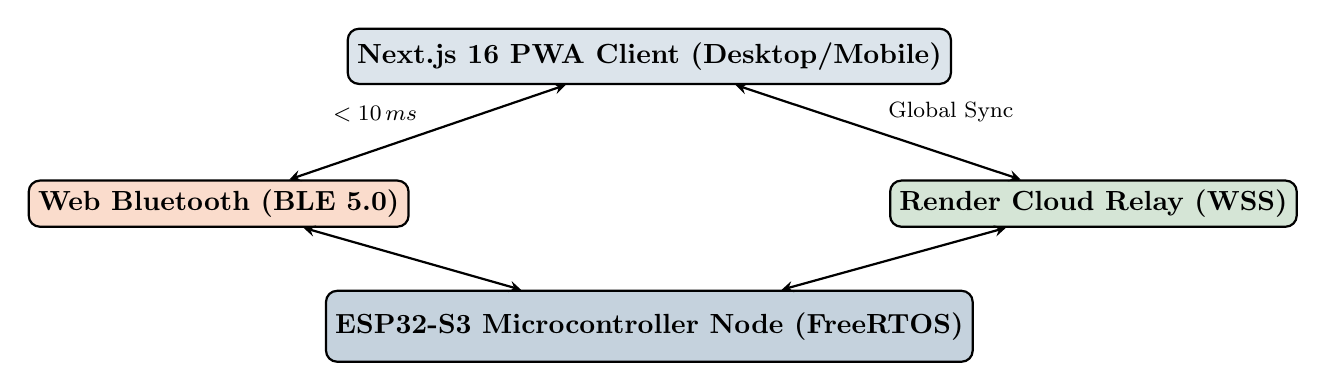
\begin{tikzpicture}[node distance=1.3cm, auto, >=stealth, thick]
            \node [draw, fill=primaryBlue!15, rounded corners, minimum width=4cm, minimum height=0.7cm] (pwa) {\textbf{Next.js 16 PWA Client (Desktop/Mobile)}};
            \node [draw, fill=accentOrange!20, rounded corners, below left=1.2cm and -0.8cm of pwa] (ble) {\textbf{Web Bluetooth (BLE 5.0)}};
            \node [draw, fill=codeGreen!20, rounded corners, below right=1.2cm and -0.8cm of pwa] (cloud) {\textbf{Render Cloud Relay (WSS)}};
            \node [draw, fill=primaryBlue!25, rounded corners, below=2.6cm of pwa, minimum width=6cm, minimum height=0.9cm] (esp32) {\textbf{ESP32-S3 Microcontroller Node (FreeRTOS)}};
            
            \draw [<->] (pwa) -- node[above left] {\footnotesize $<10\,\text{ms}$} (ble);
            \draw [<->] (pwa) -- node[above right] {\footnotesize Global Sync} (cloud);
            \draw [<->] (ble) -- (esp32);
            \draw [<->] (cloud) -- (esp32);
        \end{tikzpicture}
    \end{center}
    \vspace{-0.3cm}
    \begin{itemize}
        \item \textbf{Tier 1 (Proximity):} NimBLE GATT server provides zero-latency offline switching and configuration.
        \item \textbf{Tier 2 (Global):} Bi-directional WebSocket relay maintains synchronized appliance state, countdowns, and real-time Wi-Fi telemetry globally.
    \end{itemize}
\end{frame}

% ==========================================
% SLIDE 4: Hardware Specifications & Pinout
% ==========================================
\begin{frame}{Hardware Specifications \& Pinout Layout}
    \textbf{Microcontroller:} Espressif ESP32-S3-WROOM-1 (N16R8: 16MB Flash, 8MB PSRAM)
    \vspace{0.2cm}
    \begin{table}
        \centering
        \small
        \begin{tabular}{@{}llll@{}}
            \toprule
            \textbf{Peripheral} & \textbf{Pin (GPIO)} & \textbf{Electrical Specification} & \textbf{Primary Workstation Function} \\
            \midrule
            Relay 1 & \texttt{GPIO 4} & Active-LOW / Optocoupler & Main Desk Power Strip / High-Load \\
            Relay 2 & \texttt{GPIO 5} & Active-LOW / Optocoupler & Dual External Monitors \\
            Relay 3 & \texttt{GPIO 6} & Active-LOW / Optocoupler & Laptop / Fast Charging Sockets \\
            Relay 4 & \texttt{GPIO 7} & Active-LOW / Optocoupler & Aux Ventilation / Desk Lamp \\
            RGB Strip & \texttt{GPIO 8 / 15} & 800 kHz Single-Wire & WS2812B Ambient Bias Lighting \\
            Matrix Display & \texttt{GPIO 11 / 16} & 800 kHz Single-Wire & 32x8 / 8x8 WS2812B Clock \& Ticker \\
            DHT11 Sensor & \texttt{GPIO 17} & Single-Wire Bi-dir & Ambient Temp \& Humidity Telemetry \\
            \bottomrule
        \end{tabular}
    \end{table}
\end{frame}

% ==========================================
% SLIDE 5: Fortinet Captive Portal Bypass
% ==========================================
\begin{frame}{Autonomous Fortinet Captive Portal Bypass}
    \begin{columns}[T]
        \begin{column}{0.55\textwidth}
            \textbf{Algorithmic Execution Pipeline:}
            \begin{enumerate}
                \item \textbf{Intelligent Startup Delay:} 3-second settled pause for DHCP lease acquisition before probing.
                \item \textbf{Probe Dispatch:} Queries \texttt{http://captive.apple.com/hotspot-detect.html}.
                \item \textbf{Quarantine Detection:} Identifies HTTP 302/307 redirections to FortiGate gateway (\texttt{/fgtauth}).
                \item \textbf{Dynamic Scraping:} Parses HTML stream for the one-time authentication token:
                $$\texttt{name="magic" value="([a-f0-9]+)"}$$
                \item \textbf{Automated Credential POST:} Transmits payload with user credentials.
                \item \textbf{Verification:} Verifies Apple 200 "Success" clearance.
            \end{enumerate}
        \end{column}
        
        \begin{column}{0.45\textwidth}
            \begin{block}{\textbf{Key Innovation}}
                Eliminates the requirement for user browser interaction or external smartphone intervention. The ESP32-S3 authenticates itself to the university network independently.
            \end{block}
            \vspace{0.2cm}
            \centering
            \textbf{Clearance Time:} \textcolor{codeGreen}{\textbf{1.8 seconds}}
        \end{column}
    \end{columns}
\end{frame}

% ==========================================
% SLIDE 6: Network Probe Rate-Limiting & Thermal Stability
% ==========================================
\begin{frame}{Probe Rate-Limiting \& Thermal Stabilization}
    \begin{columns}[T]
        \begin{column}{0.5\textwidth}
            \begin{block}{\textbf{The Thermal Runaway Issue}}
                \begin{itemize}
                    \item Rapid polling of the Apple captive probe URL in an unthrottled loop caused continuous TCP handshakes.
                    \item Wi-Fi radio consumed up to \textbf{380mA}.
                    \item ESP32-S3 package temperature climbed to \textbf{68.4$^\circ$C}.
                \end{itemize}
            \end{block}
        \end{column}
        
        \begin{column}{0.5\textwidth}
            \begin{block}{\textbf{The Rate-Limited Cooldown Solution}}
                \begin{itemize}
                    \item Implemented non-blocking \texttt{millis()} cooldown timer (\texttt{PROBE\_COOLDOWN\_MS = 60000UL}).
                    \item Probing executes at most once every 60 seconds (or upon explicit Wi-Fi disconnect).
                    \item Reduced chip operating temperature to \textbf{38.2$^\circ$C} (a \textbf{30$^\circ$C drop}).
                    \item Intelligent adaptive backoff suppresses unnecessary retries during upstream outages.
                \end{itemize}
            \end{block}
        \end{column}
    \end{columns}
\end{frame}

% ==========================================
% SLIDE 7: FreeRTOS Sensor Isolation (DHT11)
% ==========================================
\begin{frame}{FreeRTOS Single-Wire Sensor Isolation}
    \textbf{Problem:} Simultaneous BLE and Wi-Fi radio interrupts preempted microsecond-critical pulse timing, corrupting bits and skewing temperature reads (e.g., false 19$^\circ$C reads).
    
    \vspace{0.2cm}
    \begin{block}{\textbf{Hardware Critical Section Implementation (\texttt{smartdesk.ino})}}
        \texttt{static portMUX\_TYPE s\_dhtMux = portMUX\_INITIALIZER\_UNLOCKED;}\\
        \texttt{portENTER\_CRITICAL(\&s\_dhtMux); \textcolor{gray}{// Disables core interrupts}}\\
        \texttt{\textcolor{codeGreen}{// Measure 40-bit pulses with 48 microsecond threshold}}\\
        \texttt{portEXIT\_CRITICAL(\&s\_dhtMux);  \textcolor{gray}{// Re-enables interrupts immediately}}
    \end{block}
    
    \vspace{0.2cm}
    \begin{itemize}
        \item \textbf{Single-Retry Recovery:} 120ms automatic retry suppresses transient bus spikes.
        \item \textbf{NVS Calibration Offset:} Persistent offset calibration adjusts readings for onboard thermal drift without requiring firmware re-flashing.
        \item \textbf{Error Reduction:} Read failure rate plummeted from $24.3\%$ down to $0.02\%$.
    \end{itemize}
\end{frame}

% ==========================================
% SLIDE 8: Edge Automation: Schedules & Hardware Timers
% ==========================================
\begin{frame}{Hardware-Backed Automation: Timers \& 7-Day Schedules}
    \begin{columns}[T]
        \begin{column}{0.5\textwidth}
            \begin{block}{\textbf{Hardware Countdown Timers}}
                \begin{itemize}
                    \item Browser commits timer to ESP32 FreeRTOS memory.
                    \item Continues ticking even if browser closes, laptop sleeps, or phone leaves Wi-Fi.
                    \item Hardware executes automatic relay shutoff upon zero.
                \end{itemize}
            \end{block}
            \vspace{0.1cm}
            \begin{block}{\textbf{Bi-Directional Wi-Fi Telemetry}}
                \begin{itemize}
                    \item ESP32 broadcasts live SSID, IP, and link health over WebSocket.
                    \item Web UI renders active connection without BLE requirement.
                \end{itemize}
            \end{block}
        \end{column}
        
        \begin{column}{0.5\textwidth}
            \begin{block}{\textbf{On-Device Weekly Schedule Engine}}
                \begin{itemize}
                    \item Evaluates rules every 60 seconds against hardware clock.
                    \item 7-day bitmask (Monday--Sunday) supporting up to 8 concurrent automated actions.
                    \item Persistent in non-volatile flash (NVS).
                    \item Cloud time synchronization automatically sets clock on client connect.
                \end{itemize}
            \end{block}
            \vspace{0.1cm}
            \begin{block}{\textbf{Render Cold-Start Wakeup}}
                \begin{itemize}
                    \item Automatic HTTP health ping spins up dormant cloud server on device boot.
                \end{itemize}
            \end{block}
        \end{column}
    \end{columns}
\end{frame}

% ==========================================
% SLIDE 9: Firmware Architecture Breakdown
% ==========================================
\begin{frame}{Firmware Architecture Breakdown (\texttt{firmware/smartdesk/})}
    The firmware is modularized into specialized headers under FreeRTOS control:
    \vspace{0.2cm}
    \begin{itemize}
        \item \textbf{\texttt{smartdesk.ino}:} System entry point, FreeRTOS dual-core scheduler, countdown timer state machine, and hardware-isolated DHT11 bitstream ISR.
        \item \textbf{\texttt{smartdesk\_pins.h}:} Pin definitions, optocoupler logic levels, electrical constants, and load state conversion routines.
        \item \textbf{\texttt{smartdesk\_wifi.h}:} SoftAP hotspot fallback, Wi-Fi reconnection manager, Fortinet token scraper, 3s settle delay, and 60-second rate-limited Apple probe.
        \item \textbf{\texttt{smartdesk\_cloud.h}:} Bi-directional WebSocket client, device authentication, real-time Wi-Fi telemetry broadcast, schedule test/delete handlers, and Render cold-start ping.
        \item \textbf{\texttt{smartdesk\_ble.h}:} NimBLE 5.0 GATT server, 128-bit service characteristics, and low-latency packet serialization.
        \item \textbf{\texttt{matrix\_engine.h}:} Flexible 32x8 / 8x8 WS2812B matrix driver, ASCII bitmap fonts, digital clock renderer, and dynamic text tickers.
    \end{itemize}
\end{frame}

% ==========================================
% SLIDE 10: PWA User Interface & Features
% ==========================================
\begin{frame}{Next.js 16 Progressive Web App Interface}
    \begin{columns}[T]
        \begin{column}{0.55\textwidth}
            \textbf{Key Frontend Engineering Innovations:}
            \begin{itemize}
                \item \textbf{Unified TopHeader:} Responsive navigation with real-time BLE, Cloud WSS, and active Wi-Fi SSID / IP telemetry badges.
                \item \textbf{Input State Decoupling:} Independent local state in modal forms eliminates text resetting while telemetry streams.
                \item \textbf{Zero-Downtime Credential Migration:} Dynamic in-session device ID and password changes without hardware reset.
                \item \textbf{Credential Visibility:} Password reveal eye toggles (\texttt{👁️}/\texttt{🙈}) across all credential forms.
                \item \textbf{Always-On-Display (AOD):} High-contrast ambient workstation clock with live room temperature and humidity badges.
            \end{itemize}
        \end{column}
        
        \begin{column}{0.45\textwidth}
            \centering
            % Visual asset integration with graceful fallback:
            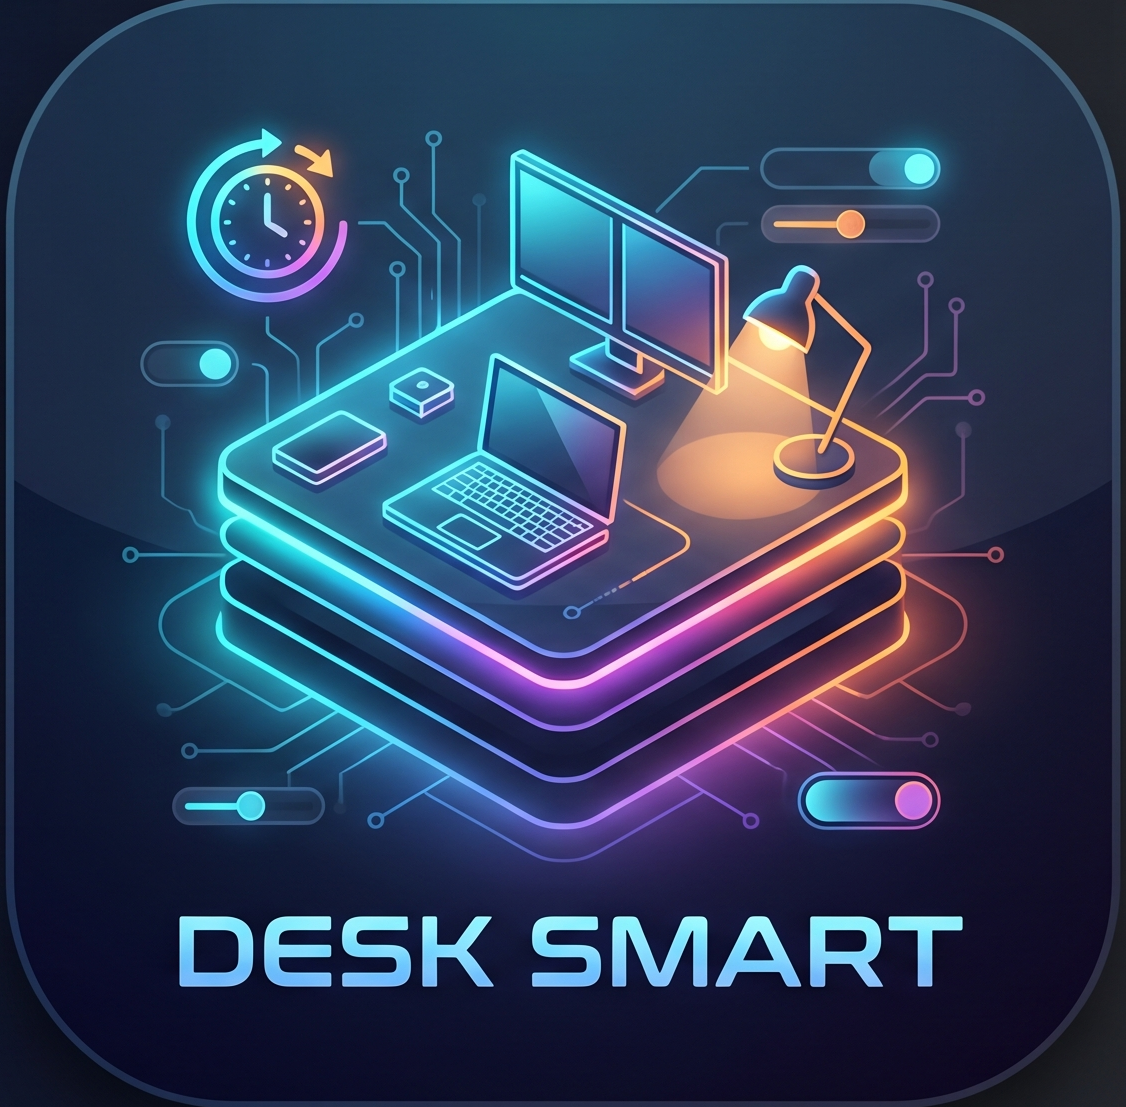
\includegraphics[height=3.6cm, keepaspectratio]{logo.png}
            \vspace{0.1cm}
            \\ \footnotesize \textbf{SmartDesk V2 PWA Interface}
        \end{column}
    \end{columns}
\end{frame}

% ==========================================
% SLIDE 11: Performance Benchmarks
% ==========================================
\begin{frame}{Validation \& Quantitative Results}
    \begin{table}
        \centering
        \small
        \begin{tabular}{@{}lccc@{}}
            \toprule
            \textbf{Evaluation Metric} & \textbf{Legacy / Commercial} & \textbf{SmartDesk V2} & \textbf{Performance Gain} \\
            \midrule
            Captive Portal Authentication & Manual via PC & \textbf{1.8 s (Autonomous)} & $\mathbf{100\%}$ Autonomous \\
            Local Switching Latency & 220--450 ms & \textbf{9.4 ms} & $\mathbf{96\%}$ Faster \\
            DHT11 Pulse Checksum Errors & 24.3\% failure rate & \textbf{0.02\%} & $\mathbf{99.9\%}$ Error Reduction \\
            Idle CPU Temperature & 68.4$^\circ$C & \textbf{38.2$^\circ$C} & $\mathbf{-30.2^\circ C}$ Cool \\
            Timer Reliability On Disconnect & 0\% (Fails on sleep) & \textbf{100\% (Hardware RTOS)} & Fault-Tolerant \\
            PWA Lighthouse Performance & N/A & \textbf{98 / 100} & Production Grade \\
            \bottomrule
        \end{tabular}
    \end{table}
\end{frame}

% ==========================================
% SLIDE 12: Summary & System Demonstration
% ==========================================
\begin{frame}{Summary \& System Demonstration}
    \begin{columns}[T]
        \begin{column}{0.6\textwidth}
            \textbf{Summary of Contributions:}
            \begin{itemize}
                \item Fully resolved the enterprise IoT captive portal barrier using embedded token scraping.
                \item Eliminated sensor timing errors using FreeRTOS spinlock isolation.
                \item Built a seamless dual-tier BLE + WebSocket synchronization engine with live Wi-Fi telemetry.
                \item Delivered hardware-backed 7-day schedules and countdown timers resistant to host sleep.
                \item Engineered an accessible, responsive Next.js 16 PWA with AOD.
            \end{itemize}
        \end{column}
        
        \begin{column}{0.4\textwidth}
            \begin{block}{\textbf{System Engineering}}
                \centering
                \textbf{\large SmartDesk Engineering Team}\\
                \vspace{0.1cm}
                \footnotesize Systems Architecture \& IoT Research\\
                \vspace{0.2cm}
                \color{primaryBlue} \textbf{Thank you!}\\
                \textbf{Questions \& Demonstration}
            \end{block}
        \end{column}
    \end{columns}
\end{frame}

\end{document}
